\chapter{Locality Sensitive Hashing}

The topic of this chapter is about techniques based on hashing that aim to construct a notion of ``distance'' from proprties of a given family of objects; practical applications include efficient grouping by using the constructed distance function, or assessing how much two objects are different from each other. The general idea of \emph{locality} is that objects that are much similar yield hashes that are almost the same, if not exactly.

Hashing typically means that an input object of great size is reduced to a much smaller ``fingerprint'', its \emph{hash}. The usual approach of constructing a distance function implementation (a \lsh-scheme), is to formulate a mathematical equation that expresses the desired notion of similarity (the distance function), and then attempt to construct an implementation using known efficient functions (the scheme). The process of creating a scheme usually involves a preprocessing step, and a function family which, by choosing one or another function according a probability distribution, statistically classifies the objects in the same way as the similarity function does.

Often, instead of looking for distance functions, the central formula models the opposite concept of \emph{similarity}. To begin, here are some common similarities for two generic subsets $A$ and $B$ (the ``objects'') taken from a universal set $U$:
\begin{align*}
    \jaccsim(A, B) =&\ \frac{|A \cap B|}{|A \cup B|}                      & \tag{Jaccard similarity} \\
    \hammsim(A, B) =&\ \frac{|A \cap B| + \abs{\overline{A \cup B}}}{|U|} & \tag{Hamming similarity}
\end{align*}

\begin{observation}
    Generally, the Jaccard similarity is more used then the Hamming similarity, because usually we have to compare sets whose size is much smaller than the size of the universe set $U$, this, using $\hammsim$, we would obtain a high similarity because of the big size of $\overline{A\cup B}$.
\end{observation}


\section{A case study: Web-page indexing}\label{sec:web-page-indexing}

This is a real-world case study that involved the search engine company Altavista in 1997; it applied an innovative technique designed by its then vice-president Andrei Broder for web-page indexing, and achieved a reduction of used storage space around a factor of 10.

The principal idea is that some kinds of documents, which are very similar to each other, are stored sparsely throughout the Internet; to save storage space, only one among the similars is picked, and its info stored in the index, while all the others are linked to the first one.

This idea is broadly captured by what is known as the \emph{Bag-of-Words} model\footnotemark, which treats bodies of text as collections of all distinct words that are contained in it. For example, given two phrases as separate bodies:

\footnotetext{\linkicon \href{https://en.wikipedia.org/wiki/Bag-of-words_model}{\textsf{Bag-of-words model --- Wikipedia}}}

\begin{itemize}
    \item $p_1 = $ \textit{``The black board is black''}
    \item $p_2 = $ \textit{``The white board is white''}
\end{itemize}

Their sets of distinct words would be those shown in figure \ref{fig:bow_venn}, where $A$ and $B$ collect respectively the distinct words of $p_1$ and $p_2$.

\begin{figure}[ht]
    \centering
    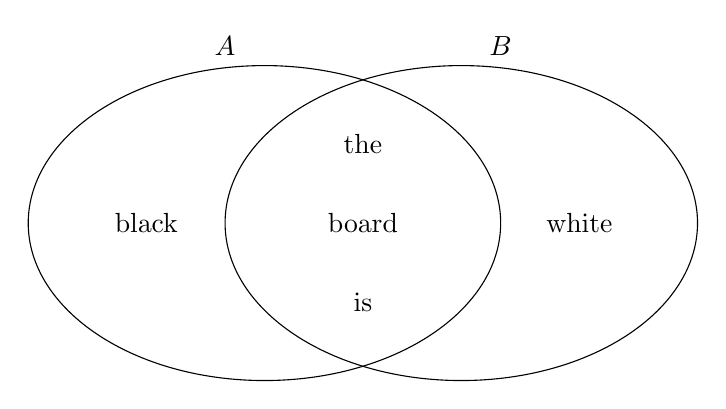
\begin{tikzpicture}

        \draw (-1.25, 0) ellipse (3 and 2) (-1.75, 2) node [above] {$A$};
        \draw (1.25, 0)  ellipse (3 and 2) (1.75, 2)  node [above] {$B$};

        \draw
            (0, 1)     node {the}
            (0, 0)     node {board}
            (0, -1)    node {is}
            (-2.75, 0) node {black}
            (2.75, 0)  node {white}
        ;
        
    \end{tikzpicture}
    
    \caption{Venn diagram of $p_1$ and $p_2$'s ``bags''}
    \label{fig:bow_venn}
\end{figure}

If the Jaccard similarity is computed on these sets, the result will be $\frac{3}{5}$. For the Hamming similarity, there is the requirement of deciding on which ``universe'' set $U$ is used as reference; in this case a sensible choice would be the collection of all existing English words (essentially, an English vocabulary), however this has the effect of bringing the similarity value extremely close to $1$. In fact, comparing all sufficiently short phrases such as $p_1$ and $p_2$, even when they do not share any word, have Hamming distance almost reaching $1$, because of the words not appearing at all; this can explain why the Jaccard similarity is a more popular choice for purposes such as in this case study.

\subsubsection{Constructing a \lsh-scheme for indexing}

The similarity of choice will then be the Jaccard similarity. The pre-processing step will be to randomly pick a permutation of all the words that appear at least once in the two bodies $\pi \in \order(A \cup B)$.

Constructing a random sequence from a given set of generic objects can be done efficiently, an example is shown in the first steps of algorithm \ref{lst:min_hash}, where words are encoded as numbers. Then the permutation $\pi$ is used to compute the hash of $A$, which consists in returning the foremost element in $A$ according to the ordering $\pi$.

\begin{lstlisting}[caption = {min hash or shingles algorithm}, label = {lst:min_hash}]
algorithm $MinHash(A)$
    // preprocessing
    $S \gets [n]$
    $\pi \gets ()$
    while $S \neq \emptyset$:
        $i \pickUAR S$
        $\pi \gets \pi \cdot (i)$               \\ intended as concatenation of sequences
        $S \gets S \setminus \{i\}$
    end
    // computing hash
    $h_\pi(A)$ := minimum element of A, according to $\pi$
    return $h_\pi(A)$
\end{lstlisting}

To prove that the steps taken to create a random ordering is effectively equivalent to picking one ordering \uar{}, observe:

\[
    \Pr[X = \pi] = \prod_{i = 1}^n \frac{1}{i} = \frac{1}{n!} = \frac{1}{\abs{\permut(A \cup B)}}
\]

The hash function may be formalized as:

\begin{equation}
    h_\pi \in \mathcal{P}(U) \to U : h_\pi(A) = min_\pi(A)
\end{equation}

Furthermore, observe that:

\[
    \forall A \subseteq U \Rightarrow h_\pi(A) \in A
\]

Back to the example, if the picked ordering is $\pi = (black, the, is, white, board)$, then the hash of $p_1$ would be $black$, while that of $p_2$ would be $the$. With a different ordering $\rho = (is, white, board, black, the)$, booth hashes would be equal: $h_\rho(p_1) = h_\rho(p_2) = is$.

It is said that $A$ is similar to $B$ if and only if $h_\pi(p_1) = h_\pi(p_2)$. Fix two objects $A$ and $B$, and focus on the ordering $\pi$. How likely is that the hashes of the two objects match? With the help of the Venn diagram in figure \ref{fig:bow_venn}:

\begin{itemize}
    \item $A \cap B = \emptyset \implies \Pr[h_\pi(A) = h_\pi(B)] = 0$; they have no words in common, so their hashes must be different, independently of the chosen order;
    \item $A = B \implies \Pr[h_\pi(A) = h_\pi(B)] = 1$; this time, all words are in common, so their hashes must coincide, again, independently of the chosen order;
    \item Otherwise, since $\pi$ is chosen \uar, the probability that the hashes are equal has the same meaning of the probability of finding the lowest element of A and B in the intersection with respect of the union (and not in $U$ as a whole, as our previous observation suggests). This is exactly the Jaccard similarity's definition:
    \todo{Formally, this doesn't add up; need to rewrite
    \[
        \Pr[h_\pi(A) = h_\pi(B)] = \frac{\Pr[\min(A) \in A \cap B \wedge \min(B) \in A \cap B]}{\Pr[\min(A) \in A \cup B \wedge \min(B) \in A \cup B]} = \frac{\abs{A \cap B}}{\abs{A \cup B}} = \jaccsim(A, B).
    \]
    }
\end{itemize}

This all happens when the ordering $\pi$ is fixed: in such a setting, the answer to question of whether two objects hash to the same value (i.e.: they are similar) will be either yes or no. The crucial improvement is to pick a subset of permutations $P$, compare the objects' hashes using each permutation, and then compute an average value as the answer; when the permutation set is sufficiently large, such answer will tend to the Jaccard similarity.

The size of $P$ required for a sufficiently good estimate can be obtained using the Chernoff bound [\ref{chernoff2}]; by setting $X_\pi$ as the random variable modeling the equality of the hashes of the objects $A$ and $B$ depending on $\pi$:

\begin{equation} \label{eq:lsh-chernoff}
    \Pr \left[ \oneover{|P|} \sum_{\pi \in P} \abs{X_\pi(A, B) - \jaccsim(A, B)} \geq \varepsilon \right] \leq 2e^{\frac{-|P| \varepsilon^2}{3}}
\end{equation}

%In other words, the difference between the average of the $X_i$ (i.e., the average of the empirically observed results) and their exact probability is greater then $\varepsilon$ only with a very small probability.

%So, how many trials (evaluations, observations) are needed to have a good estimate of the similarity? That is, what is a good value for $n$?\\
%Let $
%    X_i=\begin{cases}
%    1 & \text{if}\ h_{\pi_i}(A)=h_{\pi_i}(B)\\
%    0 & \text{otherwise}\\
%    \end{cases} $
%and $\Pr{X_i=1} = \jaccsim(A,B)=p$; we can apply the Chernoff bound on $X_i$ to compute our $n$.\\

\todo{May try to align value to new bound, and also remove some possibly unnecessary parameters like $\delta$

    If our database has $m$ pages (sets) to store, we can choose $\displaystyle |P| = \frac{\lg{\frac{2m}{\delta}}} {\varepsilon^2}$ to get a high probability of making zero errors; $\delta$ and $\varepsilon$ are parameters we can set to adjust the size of $n$: even if the bound gives us a high probability for a quite small $n$, we can choose an even smaller $n$ if we can accept big errors for very few pages.
}

We can now observe that the min hash algorithm [\ref{lst:min_hash}] is efficient: instead of comparing two entire pages, it only compares $n$ integers.

\section{A case study: Comparing DNAs}

\todo{
\textsc{Author's note}: This case is best presented with the easier notion of Hamming distance, as the similarity needs to be generalized from its presented form in order to use it here correctly; best to switch to binary strings gradually if this format is kept.
}

In the previous case study, we considered small subsets of the universe set: each web page has only few words with respect to the whole English language. However, there are cases in which the overlays between two subsets are often relevant, and this case study is one of them. Here, the Hamming similarity is significanlty preferred over the Jaccard similarity.

Let $A$ and $B$ be two sequences of \dna{} nucleotides $\{Ad, Th, Gu, Cy\}$ modeling two separate \dna{} strands of length $n$. A simple hash function would take one index value $i \in [n]$ as parameter, and return the corresponding nucleotide found in a given sequence; comparing the hashes becomes checking if the two nucleotides of their respective \dna{} sequences at the same specific positions match.

For example, define the sequences:
\begin{align*}
    A =&\ (Ad, Cy, Ad, Ad, Gu, Th, Cy, Cy) \\
    B =&\ (Gu, Cy, Th, Th, Gu, Ad, Th, Cy)
\end{align*}

then randomly pick an index value $i$, such as $8$. Then the hash function parameterized on $i = 8$ would return $Cy$ with both sequences, implying that $A$ and $B$ are similar. The probability of such two hashes being equal with respect to $i$ will turn out to be the Hamming similarity.

\todo{Probably not needed, change with something else or delete

\begin{lemma} Alternate formulation of the Hamming similarity:
    \[
        \hammsim(A, B) = 1 - \frac{\abs{A \vartriangle B}}{\abs{U}}
    \]
\end{lemma}

\begin{proof}
    \begin{align*}
        \hammsim(A, B) =&\ \frac{\abs{A \cap B} + \abs{\overline{A \cup B}}}{\abs{U}} & \\
        =&\ \frac{\abs{A \cap B} + \abs{\overline{A \cup B}} + \abs{A \vartriangle B} - \abs{A \vartriangle B}}{\abs{U}} & \\
        =&\ \frac{\abs{U} - \abs{A \vartriangle B}}{\abs{U}} & \\
        =&\ 1 - \frac{\abs{A \vartriangle B}}{\abs{U}} &
    \end{align*}
\end{proof}

\begin{align*}
    \Pr[h_i(A) = h_i(B)] &= \frac{\Pr[A[i] = B[i]]}{n} \\
    &= \frac{\Pr{(A[i] \text{ and } B[i] \text{ are both } 1) \vee (A[i] \text{ and } B[i] \text{ are both } 0 )}}{n} \\
    &= \frac{\abs{A \cap B} + \overline{\abs{A \cup B}}}{n} = \hammsim(A,B)
\end{align*}
}

Arguably, this natural arising of the Hamming similarity is most influenced by how many different ``seeds'' can be used for the hash function: in the web-page indexing case, the set of permutations of all distinct words contained in the two bodies of text grows exponentially, which justifies avoiding to use an English vocabulary from the start. Here, the index grows linearly, thus a more exaustive similarity check can be performed.

Again, the trick here is to randomly pick a subset of index values that is large enough for giving a good similarity estimate, and the Chernoff bound can provide the set size for a requested confidence level.

\subsection{Binary strings}

A closely related case study takes into consideration binary strings instead of \dna{} strands, essentially reducing the number of symmbols from 4 to 2. For example, let:
\begin{align*}
    A =&\ 010100011001 \\
    B =&\ 101111000010
\end{align*}

and pick $i = 5$ as the index value. The consequence is that the hashes are not the same, therefore the strings are considered different. With a twist of prespective, each string can be associated with a set containing the indices where the sequence has a ``1''. The probability of two hashes being equal for a given index is:

\todo{May have similar problem of formality like the previous case study

\begin{align*}
    \Pr[h_i(A) = h_i(B)] &= \frac{\Pr[A[i] = B[i]]}{n} \\
    &= \frac{\Pr{(A[i] \text{ and } B[i] \text{ are both } 1) \vee (A[i] \text{ and } B[i] \text{ are both } 0 )}}{n} \\
    &= \frac{\abs{A \cap B} + \overline{\abs{A \cup B}}}{n} = \hammsim(A,B)
\end{align*}
}


\section{LSH formalization}

% The generic steps that have been taken in all case studies is to turn the objects of interest (bodies of text, \dna{} strands, binary strings) into subsets of nonnegative integers, according to some simple rules of choice; web-pages may be turned into Bag-of-Words and then into number subsets using a lexicographical map,  and binary strings to the sets containing all indices that have a 1. In this sense, the universe set is effectively always the power set of $\nonneg$

% Note: Might want to complete the hash function picture by including their use in cryptography, where the purposes and methods are wildly different
% Note: Actually, might want to modify the definitions, especially around hash functions, bringing them closer to the typical definitions in crypto; maybe using the seed S as an RV in calculations will make the rest more understandable

First let us focus around the hash function as an object: its true purpose in a scheme is to classify objects based on how much they ``look like'', whatever this means in the chosen similarity's terms. Therefore, in our theoretical analysis, the codomain of a hash function is not that important; what is important is how the function partitions its own domain, $U$. In a sense, we're interested only in the partitions of $U$ themselves, not in the functions that generate them.

Why have we dealt with functions back then? Moving from a purely mathematical perspective to a more computational one, what is usually done for measuring similarities is sampling some object's characteristics, and observe how ``distant'', or else ``similar'' they are. This is done by means of some program; and programs are (oh so) easily associated with functions. The computational approach gives a more practical vision of the problem we're confronting ourselves with.

In spirit of such practical perspective, the following mathematical definitions are kept with functions, and a generic fingerprint/signature/hash space $\Theta$ will be used as the codomain throughout the chapter.

% Old note: what could happen, is to have a couple of functions that map values into wildly different codomains, but partition $U$ in exactly the same way! And in our journey, we're just interested in classifying objects; so these kind of ``duplicate'' functions are, well, useless (unless we delve in complexity studies, but that's out of our scope).


% TODO Still incomplete, need the trineq on 1-S
\begin{definition}
    Let $U$ be a set, and $f \in U^2 \to [0, 1]$ a symmetric function; then $f$ is called a \emph{similarity} over $U$.
\end{definition}

\todo{May need more details around the seed $s$}
\begin{definition}
    A \lsh-scheme over $U$ is a hash function family $h_s \subseteq (U \to \Theta)$, where $s$ is picked according to a probability distribution; in general $\abs{\Theta} \ll \abs{U}$
    
    Alternatively, given a universe $U$, a function $S \in U^2 \to [0, 1]$ is said to be a \emph{\lsh-able similarity} if and only if there exists a distribution over a hash function family $h_s \subseteq (U \to \Theta)$ such that: 
    \begin{equation}
        \forall X, Y \in U \qquad \Pr[h_s(X) = h_s(Y)] = S(X, Y)
    \end{equation}
\end{definition}

\begin{example}
    We can apply the min-hash scheme [\ref{lst:min_hash}] to the Jaccard Similarity. With $U = [3]$ and seed $\pi = 1 < 2 < 3$, the function partitions its domain into 4 blocks:
    \begin{align*}
        \emptyset                           &\mapsto \perp \text{(the hash of the empy set is a special symbol)} \\
        \{1\}, \{2,1\}, \{1,3\}, \{1,2,3\}  &\mapsto 1 \text{ (all sets containing 1 have hash 1)} \\
        \{2\}, \{2,3\}                      &\mapsto 2 \text{ (all remaining sets containing 2 have hash 2)} \\
        \{3\}                               &\mapsto 3 \text{ (all remaining sets containing 3 have hash 3)}
    \end{align*}
\end{example} 

\begin{example}
    Similarly, we can apply the function based on the Hamming Similarity we saw in the binary strings' case to the same set $U = [3]$. Picking $i = 2$ as the seed, this time the function induces a bipartition:
    \begin{align*}
        \{2\}, \{2.1\}, \{2,3\}, \{1,2,3\}  &\mapsto 1 \text{ (all sets containing $i$ have hash 1)} \\
        \emptyset, \{1\}, \{3\}, \{1,3\}    &\mapsto 0 \text{ (all remaining sets have hash 0)}
    \end{align*}
\end{example}


% INSIGHT
\obs Preprocess and hash function (aka a scheme) determine the similarity function; in real world scenarios, attempts are made to construct such elements to implement such similarity

% MAJOR INSIGHT:
\obs In the previous webpage example [\ref{sec:web-page-indexing}], we're not dealing with a single hashing function, but with a family of functions each built with its own word permutation: the scheme distributes over the permutations of the union!
% Now, do all permutations induce unique partitions? AP200828: Good question, might be true considering the domain being \powerset{\nonneg}


\begin{proposition} \label{ex:transitivity}
    There exist similarities that cannot have \lsh-schemes.
\end{proposition}

\begin{proof}
    Let $f$ be the similarity:
    \begin{align*}
        f(a, b) = 1 \\
        f(b, c) = 1 \\
        f(a, c) = 0
    \end{align*}

    and let $h_s$ be an arbitrary function family implementing it. Since $f(a, b) = f(b, c) = 1$, it entails that $h_s(a) = h_s(b) = h_s(c)$ which contradicts the third mapping of $f$.
\end{proof}


\subsection[\texorpdfstring{The $\gamma$-similarity}{The gamma-similarity}]{The $\bm\gamma$-similarity}

Other similarities akin to $\jaccsim$ have been designed:
\begin{align*}
    D(A, B)  =&\ \frac{\abs{A \cap B}}{\abs{A \cap B} + \frac{1}{2} \abs{A \vartriangle B}} & \tag{S\o{}rensen-Dice similarity} \\
    An(A, B) =&\ \frac{\abs{A \cap B}}{\abs{A \cap B} + 2 \abs{A \vartriangle B}}           & \tag{Anderberg similarity}
\end{align*}

and they can be collectively expressed with a single similarity function parameterized on $\gamma$:

\begin{definition}[$\gamma$-similarity]
    \begin{equation}
    \displaystyle S_\gamma(A, B) = \frac{\abs{A \cap B}}{\abs{A \cap B} + \gamma \abs{A \vartriangle B}}
    \end{equation}
\end{definition}

In this perspective:
\begin{align*}
    \jaccsim =&\ S_1 \\
    D        =&\ S_\frac{1}{2} \\
    An       =&\ S_2
\end{align*}

It would be useful to know for which values of $\gamma$ there exists an LSH for $S$; the next lemma helps us finding an answer:

\begin{lemma}[Charikar] \label{lem:charikar}
    If a similarity $S$ admits a \lsh-scheme, then the function $d = 1 - S$ must satisfy the triangular inequality; thus, $d$ is a metric\footnote{In most cases, similarities are actually defined as inverses of some existing metric.}:
    \[
        \forall A, B, C \in U \quad d(A, B) \leq d(A, C) + d(B, C)
    \]
\end{lemma}

\begin{proof}
    Let $A$, $B$ and $C$ be three objects; consider how their hashes may differ to each other in all possible ways as shown in the following table, and associate each combination to a probability $p_i$:
    
    \vspace{1ex}
    \begin{tabular}{lllll}
              & $A \not\sim B$ & $A \not\sim C$  & $B \not\sim C$  & may exist \\
        $p_1$ & T          & T           & T           & \correct  \\
        $p_2$ & T          & T           & F           & \correct  \\
        $p_3$ & T          & F           & T           & \correct  \\
        $p_4$ & T          & F           & F           & \error    \\
        $p_5$ & F          & T           & T           & \correct  \\
        $p_6$ & F          & T           & F           & \error    \\
        $p_7$ & F          & F           & T           & \error    \\
        $p_8$ & F          & F           & F           & \correct
    \end{tabular}

    Observe that some combinations cannot happen because of internal contradictions, violating proposition [\ref{ex:transitivity}]; they are marked with \error{} for reference. In such cases, their probability of happening will be $0$.
    Computing the distances between the objects with $d$:
    \begin{align*}
        d(A, B) &= 1 - S(A, B) = \Pr[A \not\sim B] = p_1 + p_2 + p_3 + p_4 \\
        d(A, C) &= 1 - S(A, C) = \Pr[A \not\sim C] = p_1 + p_2 + p_5 + p_6 \\
        d(B, C) &= 1 - S(B, C) = \Pr[B \not\sim C] = p_1 + p_3 + p_5 + p_7
    \end{align*}
    
    Using such mappings in the triangular inequality, and knowing that some of the probabilities are $0$:
    \begin{align*}
        d(A, B)         &\leq d(A, C) + d(B, C) \\
        p_1 + p_2 + p_3 &\leq 2p_1 + p_2 + p_3 + 2p_5 \\
        0               &\leq p_1 + 2p_5
    \end{align*}

    which is true for any values $p_1$ and $p_5$. Therefore, the triangular inequality is satisfied, $d$ is a metric, and $S$ admits a \lsh-scheme.
\end{proof}

\begin{corollary}
    Dice's similarity cannot admit a \lsh-scheme.
\end{corollary}

\begin{proof}
    This proof goes by counterexample. Assume $A = \{1\}, B = \{2\}, C = \{1, 2\}$, then use the triangular inequality over the distances:
    \begin{align*}
        & D(A, C) = \frac{2}{3},\ D(B, C) = \frac{2}{3},\ D(A, B) = 0 \\
        & d(A, B) = 1 - D(A, B) = 1 > \frac{2}{3} = (1 - D(A, C)) + (1 - D(B, C)) = d(A, C) + d(B, C)
    \end{align*}
    A contradiction is reached, thus $d$ is not a metric. By Charikar's lemma, $D$ cannot admit a \lsh-scheme.
\end{proof}

The counterexample also sheds some insight on $\gamma$-similarities: a bound on $\gamma$ for \lsh-able functions can be obtained. Let $A = \{1\},\ B = \{2\},\ C = \{1, 2\}$ and $S_\gamma(A, C) = \frac{1}{1 + \gamma},\ S_\gamma(B, C) = \frac{1}{1 + \gamma},\ S_\gamma(A, B) = 0$. Then:
\begin{align*}
    1 =&\ 1 - S_\gamma(A, B) 							& (S_\gamma(A, B) = 0) \\
      >&\ (1 - S_\gamma(A, C)) + (1 - S_\gamma(B, C)) 	& \text{(trineq on $1 - S_\gamma$, which is a metric by lemma \ref{lem:charikar})} \\
      =&\ 2 \left( 1 - \frac{1}{1 + \gamma} \right)		& \\
      =&\ \frac{2\gamma}{1 + \gamma} 					&
\end{align*}

which entails:
\[
    1 > \frac{2\gamma}{1 + \gamma} \quad \implies \quad \gamma < 1
\]
Hence, if $\gamma < 1$, the triangular inequality does not hold, so no \lsh-scheme can be designed.

    
\section{Probability generating functions}

\begin{definition}

    Given a discrete random variable $X$, its corresponding \emph{probability generating function} (\pgf{} in short), is a power series representation of $X$:
    \[
        \pgfunc_X(\alpha) = \sum_{x = 0}^{\infty} \Pr[X = x] \alpha^x
    \]

    Note that all outcomes appear by their probability.
\end{definition}

To get back to the corresponding probability mass function:
\[
    \Pr[X = \omega] = \frac{\mathcal{D}_x^\omega(\pgfunc_X)(0)}{x!}
\]
where $\mathcal{D}_x^\omega$ denotes the $\omega$-th derivative on $x$.


\subsection{Constructing schemes from \pgf{}s}

New similarities can be defined by applying a \pgf on them; this comes in very handy if such similarity admits a \lsh-scheme from the beginning:

% TODO check
\todo{Can we just prove that probability distributions are composable? lshability could be just a carried-over property...

AP200829: Similarities --are not-- distributions; however the lsh-schemes that implement them are, in a sense}

\todo{This asks for a formal way to say that a similarity can have a scheme}

\begin{theorem} \label{thm:pgfcompsim}
    Let $S$ be a similarity $S$ that admits a \lsh-scheme, and $f$ a \pgf:
    \[
        f(S) \in (U^2 \to [0, 1]) : (A, B) \mapsto f(S(A, B))
    \]
    then $f(S)$ is \lsh-able. More concisely:
    \[
        f(S(A, B)) = (f(S)) (A, B)
    \]
\end{theorem}


The proof is inductive and makes use of four lemmas presented here. The first one forms the basis of induction:


\begin{lemma}\label{lem:pgfcomp}
    If $S$ and $T$ are similarities over $U$ that have a scheme, then $S \cdot T : (S \cdot T)(A, B) = S(A, B) \cdot T(A, B)$ has a scheme. In other words, \lsh-ability is preserved on concatenation.
\end{lemma}

\begin{proof}
    Let $h_s$ and $j_t$ be two hash functions that respectively implement the similarities $S$ and $T$. Construct a new function $k_{(s, t)}$:
    \[
        k_{(s, t)} \subseteq (U \to \Theta_S \times \Theta_T) : A \mapsto (h_s(A), j_t(A))
    \]

    Then, for any objects $A$ and $B$:
    \begin{align*}
         &\ \Pr[k_{(s, t)}(A) = k_{(s, t)}(B)]              & \\
        =&\ \Pr[h_s(A) = h_s(B) \wedge j_t(A) = j_t(B)]     & \\
        =&\ \Pr[h_s(A) = h_s(B)] \cdot \Pr[j_t(A) = j_t(B)] & (s \indep t) \\
        =&\ S(A, B) \cdot T(A, B)                           &
    \end{align*}

    which means that $k_{(s, t)}$ is effectively a \lsh-scheme for the similarity $S \cdot T$.
\end{proof}

\begin{lemma}\label{l:powersim}
    If $S$ is a \lsh-able similarity, then so is $S^i$ for any nonnegative integer $i$.
\end{lemma}

\begin{proof}
    The \lsh-able similarity used to prove the lemma is a trivial one $O$ that treats all objects as equivalent to each other, and its scheme is easily implemented by a constant hash function:
    \begin{align*}
        O         \in&\ U^2 \to [0, 1]    : & O(A, B) \mapsto 1 \\
        h_s \subseteq&\ U \to \mathbbm{1} : & A \mapsto 0
    \end{align*}

    This forms the base step of the proof by induction, for $i = 0$. The inductive step consists in proving that $S^{i + 1} = S \cdot S^i$ admits a \lsh-scheme for any $i$, and since $S$ does admit one by definition, $S^i$ does admit one too by inductive hypothesis, and lemma \ref{lem:pgfcomp} proves that \lsh-ability is preserved upon concatenation, $S^{i + 1}$ does admit a \lsh-scheme, completing the proof.
\end{proof}

\begin{lem}[L4]\label{l:pgf_4}
    Let $P = \{p_i\}$ be a countably infinite set of real numbers between 0 and 1 such that their total sum is 1, and $S = \{S_i\}$ be a set of \lsh-able similarities such that $\abs{S} = \abs{P}$. Then $\sum_{i = 0}^{\infty} p_i S_i$ is also a \lsh-able similarity.
\end{lem}

\begin{proof}

    \todo{Something's off: \pgf{}s require a single $\alpha$ that is exponentiated in the definition, but here there are "multiple" alphas. Maybe there should be a "selecting function" that, by repeated applications, yields the similarity of interest? Can this be done correctly?

    Also, for the theorem's proof, this is too strong: a single similarity instead of a generic collection is enough, and the statement becomes much simpler to prove

    Proven by construction:
    \begin{enumerate}
        \item First, sample $j$ at random from $\nonneg$ with probability $p_0, ..., p_i, ...$;
        \item Then, sample $h$ from the hash functions (LSH) of $S_j$ (that is, we are choosing which LSH to use);
    \end{enumerate}
    Therefore:
    \begin{align*}
        &\  \Pr_h[h(A) = h(B)] \\
        =&\ \sum_{i = 0}^{\infty} p_i S_i(A, B) \\
        =&\ \sum_{i = 0}^{\infty} \Pr[i = j] \Pr_h[h(A) = h(B) \knowing i = j] \qedhere
    \end{align*}
    }
\end{proof}

This lemma is useful if a weighted average is needed:
\[
    W(A,B) = \sum_{i=0}^{\infty}(p_i S_i(A, B))
\]

\begin{proof}[Proof of the theorem \ref{thm:pgfcompsim}]
    We want to prove that $\sum_{i = 0}^{\infty} p_i S^i$ has a scheme. By lemma [\ref{l:powersim}] we know $S^i$ has a scheme, and by L4 [\ref{l:pgf_4}] we know the sum is lshable.
\end{proof}


\subsubsection{Use cases}

This theorem is much valuable when constructing a \lsh-scheme: the principal technique is to concatenate the results of different hash functions from different similarities, while keeping a small fingerprint.
\[
    f(x) = \sum_{i=1}^{a}(2^{-i} \cdot x^i)
\]

For instance, Another consequence of the theorem is revealed when the statement is applied to the Jaccard similarity.

Our function is $f_\gamma$, with $\gamma > 1$, defined as
\begin{equation} \label{eq:pgf_jacc}
    f_\gamma(x) = \frac{x}{x + \gamma(1 - x)}
\end{equation}

In order to prove $f_\gamma$ is a \pgf, we have to prove that the coefficients represent a probability distribution: they are all positive and their sum is 1. By applying the Taylor series expansion to [\ref{eq:pgf_jacc}], we get:
\todo{No idea on how to get there... :(}
\[
    f_\gamma(x) = \sum_{i = 1}^{\infty} \frac{ \left( 1 - \frac{1}{\gamma} \right)^i }{\gamma - 1} x^i
\]

now $f_\gamma$ is a power series, so all the coefficients are positive. By applying the sum-to-1 hypothesis, it is to prove that:
\[
    \sum_{i = 1}^{\infty} \frac{ \left( 1 - \frac{1}{\gamma} \right)^i }{\gamma - 1} = 1 \qquad \implies \qquad \sum_{i = 1}^{\infty} \left( 1 - \frac{1}{\gamma} \right)^i = \gamma - 1
\]

And indeed:
\begin{align*}
        \sum_{i = 1}^{\infty} \left(1 - \frac{1}{\gamma} \right)^i
    =&\ \left( 1 - \frac{1}{\gamma} \right) \sum_{i = 0}^{\infty} \left( 1 - \frac{1}{\gamma} \right)^i & \text{(adding finite terms to an infinite series)} \\
    =&\ \left( 1 - \frac{1}{\gamma} \right) \frac{1}{1 - \left( 1 - \frac{1}{\gamma} \right)}           & \text{(geometric series with $\alpha < 1$)} \\
    =&\ \frac{\gamma - 1}{\gamma} \cdot \frac{1}{ \left( \frac{1}{\gamma} \right) }                     & \\
    =&\ \gamma - 1                                                                                      &
\end{align*}

Therefore $f_\gamma$ is a \pgf. Applying it to the Jaccard similarity:
\begin{align*}
        f_\gamma (\jaccsim(A, B))
    =&\ f_\gamma \left( \frac{\abs{A \cap B}}{\abs{A \cup B}} \right) \\
    =&\ \frac{\frac{\abs{A \cap B}}{\abs{A \cup B}}} {\frac{\abs{A \cap B}}{\abs{A \cup B}} + \gamma \frac{\abs{A \cup B} - \abs{A \cap B}}{\abs{A \cup B}}} \\
    =&\ \frac{\abs{A \cap B}} {\abs{A \cap B} + \gamma \abs{A \vartriangle B}} \\
    =&\ S_\gamma(A, B)
\end{align*}

which in turn, by theorem \ref{thm:pgfcompsim}, is \lsh-able.


\section{Sketches}

Sketches are an alternative method to \lsh-schemes for the concept of  represent bigger and more comlpex objects using just a few selected properties. Note that this is not akin to a compression method, which seeks to exactly map an original object with a unique, smaller image

\begin{example}
    It's possible to go back to $\abs{A \cap B}$ from data such as $\abs{A}$, $\abs{B}$, $h_s(A)$, $h_s(B)$ and $\jaccsim(A, B) \pm \varepsilon$. Note that the similarity value can be obtained from the objects' hashes by applying the Chernoff bound, and all other data need just a few additional bits to be stored.
\end{example}

\begin{example}
    It's possible to approximate $\frac{\abs{A \cap B}}{\abs{A \cap B} + \frac{1}{2}\abs{A \vartriangle B}}$ with $\frac{1}{2} \cdot \abs{A \cup B} + \frac{1}{2} \cdot \abs{A \cap B}$.
\end{example}

% TODO check
% --------------------------------------------------------------
% ??sorensen dice??cosine similarity?? inner product??johnson-lindenstrauss??
    
%a sketch is n instance of a pgf which can be used to implement other similarities NONONONONOO
    
    
    
\subsection{Sketching non-\lsh-able similarities}

Sketching proves to be invaluable in that it is able to make good enough approximations of similarities that do not admit a \lsh-scheme; the starting point is usually a \lsh-scheme from another similarity. For example, it is possible to approximate $S_\gamma$ with $\jaccsim$ with an error of $\frac{1}{\gamma}$.

\todo{What's the point here?}
\begin{example}
    Let $f$ be a \pgf, and $\alpha \sim \berdist(p)$. Define the following function:
    \[
        f_\alpha(S) = \begin{cases}
            \alpha \cdot f(S)		& \text{with probability $p$} \\
            (1 - \alpha) \cdot T	& \text{with probability $(1 - p)$}
        \end{cases}
    \]

    where $S$ is a similarity grouping every element under a single class, and $T$ is another smiliarity where each element has its own distinct class.

    When $\alpha = 1$, $f_\alpha$ induces a banal partition over its domain, whereas with $\alpha = 0$ the induced partition is punctual. The hash functions that can implement such a function would be a constant one for $S$, and an identity function for $T$ (remember that in $T$'s case, $T(x, x) = 1$). However this is not a good scheme, because we're not shrinking data.

\end{example}

\begin{definition}[Distortion]
    Given a similarity $S$, it is said to have a \emph{distortion} at most a value $\delta \geq 1$ if and only if there is a similarity $T$ defined on the same universe, such that $T$ admits a \lsh-scheme, and:
    \[
        \frac{S}{\delta} \leq T \leq S.
    \]
\end{definition}

The most relevant property of a distorted similarity is that it globally underestimates the original similarity; in the extreme (and arguably unlikely) case, all objects would result non-similar to each other.

Note that $\delta$ acts as an \emph{approximation factor}, and the more it approaches $1$, the more $T$ gets closer to $S$; at the limit $\delta = 1$, $S$ does admit a \lsh-scheme by itself.

\todo{Something's wrong: both gamma and delta are said to be at least 1}
For example, where we used $\jaccsim$ to approximate $S_\gamma$, we had $\delta \to \frac{1}{\gamma}$. To check if there is a better approximation, the following lemma is presented:

\begin{lemma}[Center lemma] \label{lem:center}
    Let $S$ be a \lsh-able similarity, and $V$ a subset of $U$ in which all elements are exactly non-similar, which will be called a \emph{partial section} of $S$:
    \[
        \forall A, B \in V \qquad S(A, B) = 0
    \]
    Then:
    \[
        \forall A \in U \qquad \sum_{B \in V} S(A, B) \leq 1
    \]
\end{lemma}

\begin{proof}

    \todo{Here the idea of modeling the seed as a RV finally pops out of nowhere... need to review all of the chapter on all probabilities
    
    A concern about picking seeds with positive probabilities is raised too, which isn't much valuable, hash function families really need a section of their own in this chapter}
    Fix an object $A \in U$, and let $h_X$ be a \lsh-scheme for $S$ with the seed $X$ as a random variable. Then:
    \begin{align*}
            &\ \sum_{B \in V} S(A, B)                                                                       & \\
           =&\ \sum_{B \in V} \Pr[h_X(A) = h_X(B)]                                                          & \text{(S is \lsh-able)} \\
           =&\ \sum_{B \in V} \sum_{X \in \mathcal{S}} \Pr[X = x] \cdot \Pr[h_X(A) = h_X(B) \knowing X = x] & \text{(Total prob. on the seeds of $h_X$)} \\
           =&\ \sum_{X \in \mathcal{S}} \Pr[X = x] \cdot \sum_{B \in V} \Pr[h_x(A) = h_x(B)]                & \text{(Condition collapse)} \\
        \leq&\ \sum_{X \in \mathcal{S}} \Pr[X = x]                                                          & \text{(Any prob. is between 0 and 1)} \\
           =&\ 1                                                                                            &
    \end{align*}
\end{proof}

Some trivial but interesting consequences are:

\begin{corollary}
    The average similarity between any object in $U$ and an object in a partial section $V$ of $U$ is at most $\frac{1}{\abs{V}}$.
\end{corollary}

\begin{corollary}\label{cor:center}
    \[
        \exists A \in V \forall B: S(A, B) \leq \frac{1}{\abs{V}}
    \]
\end{corollary}


\subsubsection{Application to $S_\gamma$}

\todo{Feels weak}
    
We will now prove what we said about $S_\gamma$'s approximation using the lemma we have just proven. The framework will be:

\begin{itemize}
    \item $S := S_\gamma \text{, with } 0 < \gamma < 1$,
    \item $U := \powerset([n])$,
    \item $V := \powerset_1([n])$;
\end{itemize}

$\powerset_1([n])$ satisfies the definition of partial section for $S_\gamma$ (it is actually a complete one), because all singletons are disjoint, and thus any similarity computed between any two of them will evaluate to 0. Let $T$ (that will be our $S'$) be a \lsh-able similarity that finitely distorts $S_\gamma$; then for any two singletons $A$ and $B$ in $\powerset_1([n])$ $T(A, B)$ will also be always zero, since $T$ undervalues $S_\gamma$ by definition. Since $T$ is also \lsh-able, the center lemma can be applied:
\begin{align*}
    \oneover{\delta} S_\gamma(A, B)                     \leq&\ T(A, B) \leq S_\gamma(A, B)      & \text{(by definition of distortion)}\\
    \oneover{\delta} \cdot \oneover{1 + \gamma (n - 1)} \leq&\ T(A, B) \leq \oneover{n}         & \text{(by definition of $S_\gamma$ and corollary \ref{cor:center})} \\
    \delta (n \gamma - \gamma + 1)                      \geq&\ n                                & \\
    \delta                                              \geq&\ \frac{n}{n \gamma - \gamma + 1}  &
\end{align*}

The point of interest here is that, as $n$ tends to infinity, $\delta$ approaches $\frac{1}{\gamma}$; the conclusion is that the distortion bound of $S_\gamma$ is indeed $\frac{1}{\gamma}$.


\subsubsection{Application to the cosine similarity}
\todo{Not reviewed yet}

Now we would like to apply the same method to the \emph{cosine similarity}, also known as the \emph{inner product similarity}.  Let's start again with some definitions:

\begin{itemize}
    \item $U := \{ \vec{x} \ | \ \vec{x} \in \mathbb{R}_+^n, \ \abs{\abs{\vec{x}}}_2=1 \}$ \ \
    (i.e., $U$ is a positive hypersphere with the center in the origin and the radius equal to 1),
    \item $C \in U^2 \to [0,1]$ s.t. $C(\vec{x}, \vec{y}) = \left\langle \vec{x}, \vec{y} \right\rangle = \sum_{i=1}^n x_iy_i$;
\end{itemize}

Now, we want to know if $C$ has an LSH and, if not, what is its distortion. Define:
\[
    \mathcal{X}=\{ \vec{x}_1, \vec{x}_2, ..., \vec{x}_n \} \text{ , where } x_i(j)=\begin{cases}
        1 & \text{if } i = j \\
        0 & \text{otherwise} \\
    \end{cases} 
\]
or in other terms, $\vec{x}_i=(0,...,0,1,0,...,0)$ with the only 0 in position $i$. Then:

\begin{itemize}
    \item So we have that $\abs{\abs{\vec{x}}}_2=\sqrt{1^2+0^2(n-1)}=1$;
    \item Moreover $C(\vec{x_i}, \vec{x_j})=0 \ \forall i\neq j$;
    \item Let $\vec{y}=\left( \underbrace{\frac{1}{\sqrt{n}}, \frac{1}{\sqrt{n}}, ..., \frac{1}{\sqrt{n}}}_\text{n times} \right)$, then $\abs{\abs{\vec{y}}}_2 = \sqrt{\sum_{i=1}^n y_i^2} = \sqrt{\sum_{i=1}^n \frac{1}{n}}=1$;
    \item So, $C(\vec{x_i}, \vec{y})= \sum_{j=1}^n \left( x_i(j) \cdot y_i(j) \right) = x_i(i) \cdot y_i(i) = \frac{1}{\sqrt{n}}$;
    \item Then $\delta \geq \sqrt{n}$, so, unlike before, the distortion is big and grows bigger with $n$.
\end{itemize}

Some other related examples follow:

\begin{example}
    \emph{Weighed Jaccard} is a generalization of $\jaccsim$ for vectors: \\ $\mathcal{WJ}=\frac
    {\sum_i \min(x_i, y_i)}{\sum_i \max(x_i, y_i)}$.
\end{example}

\begin{example}
    \textbf{Sim Hash} is an LSH scheme similar to the cosine similarity:
    \begin{itemize}
        \item $\mathcal{CS}(\vec{x},\vec{y})=
            \cos(\theta_{\vec{x},\vec{y}}) $;
        \item $\mathcal{SH}(\vec{x},\vec{y})=
            1-\frac{\theta_{\vec{x},\vec{y}}}{\pi} $;
        \item $\mathcal{SH}$ is high if the angle $\theta$ is small;
        \item $\frac{\theta_{\vec{x},\vec{y}}}{\pi}$ is the probability that an hyperplane divides $\vec{x}$ and $\vec{y}$, where the hyperplane is a threshold between similar and dissimilar elements of the universe, so it creates a partition of the universe in two sets.
    \end{itemize}
\end{example}

